\chapter{Resultados e Discussões}
\label{cap:resultados}

Neste capítulo, apresentam-se os resultados quantitativos e qualitativos obtidos a partir da execução do pipeline computacional desenvolvido. Inicialmente, realiza-se uma análise exploratória dos sinais de vibração e da relevância física dos atributos extraídos. Na sequência, avalia-se comparativamente o desempenho dos modelos \textit{Random Forest} e \textit{Support Vector Machines} nos cenários de validação cruzada agrupada e teste independente. Por fim, analisam-se as matrizes de confusão e a eficácia da estratégia de votação majoritária por ensaio sob a perspectiva da dinâmica de vibrações mecânicas.

\section{Análise Exploratória dos Sinais e Atributos}
\label{sec:analise_exploratoria}

A \autoref{fig:sinais_tempo_fft} ilustra o comportamento comparativo entre uma série temporal correspondente a um rolamento íntegro (\texttt{Normal\_0.mat}) e um rolamento com defeito severo de \SI{0.021}{in} na pista interna (\texttt{IR021\_0.mat}), ambos operando sob rotação nominal de \SI{1797}{rpm} (carga nula).

\begin{figure}[htbp]
    \centering
    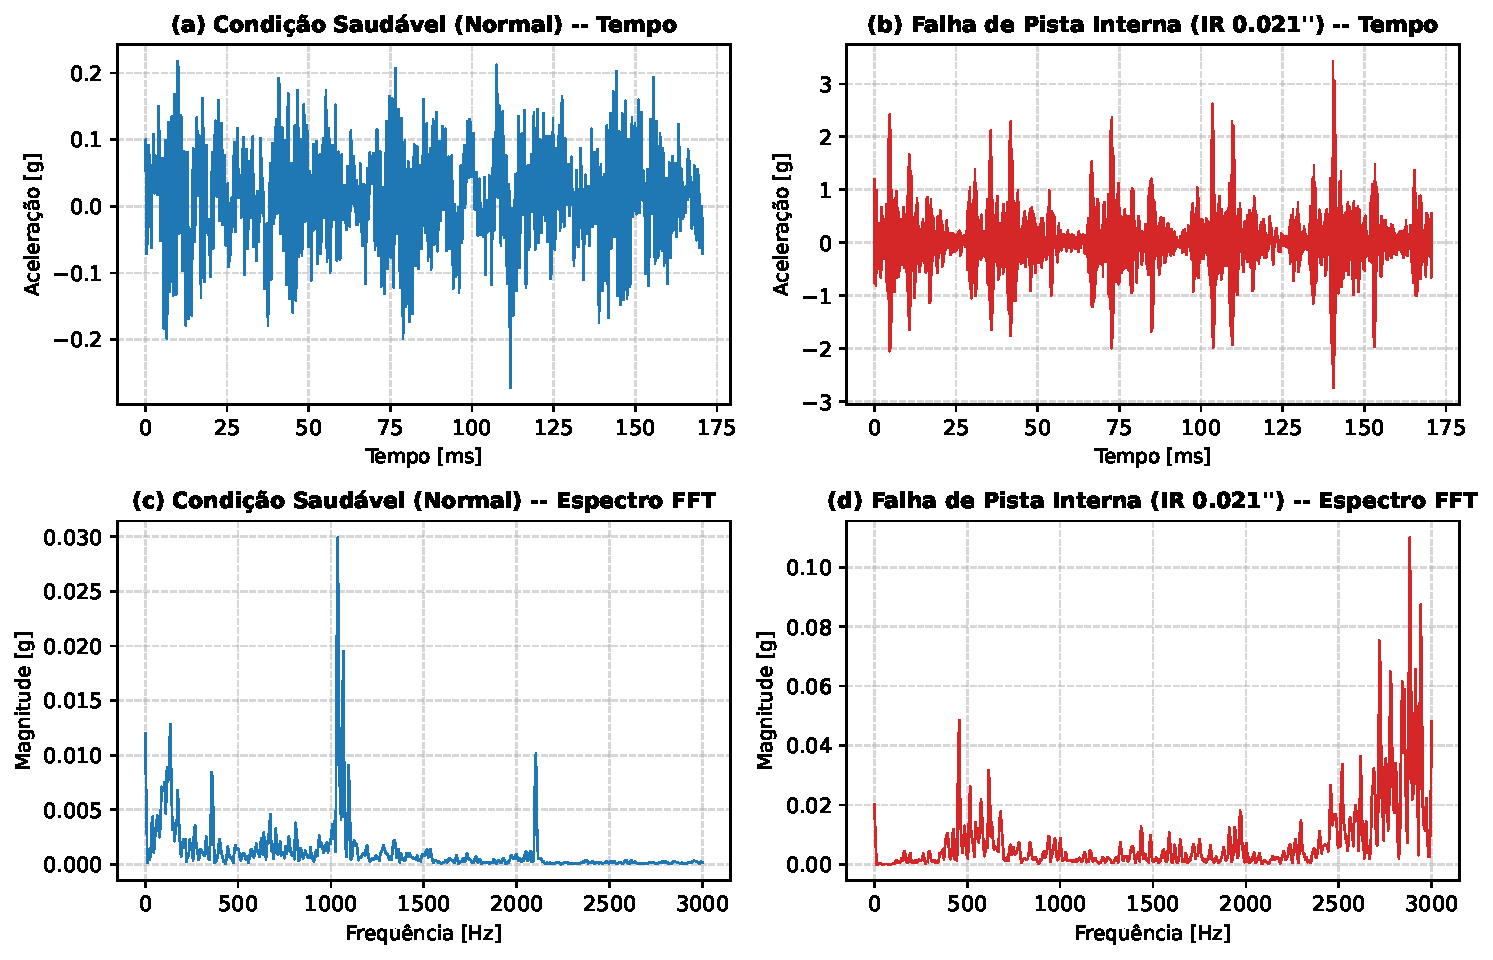
\includegraphics[width=0.98\textwidth]{fig_sinais_tempo_fft.pdf}
    \caption{Comparativo no domínio do tempo e no domínio da frequência (FFT com janela de Hanning) entre rolamento saudável e com falha na pista interna}
    \label{fig:sinais_tempo_fft}
    \legend{Fonte: Elaborado pelo autor (2026).}
\end{figure}

A inspeção da \autoref{fig:sinais_tempo_fft}(a) evidencia que o rolamento saudável exibe um perfil vibratório de baixa amplitude, confinado na faixa de $\pm \SI{0,15}{g}$, com comportamento estocástico aproximadamente gaussiano gerado pelo ruído mecânico basal do motor e desbalanceamento residual mínimo. Seu respectivo espectro FFT (\autoref{fig:sinais_tempo_fft}(c)) apresenta magnitudes uniformemente reduzidas ($< \SI{0,01}{g}$) em todo o espectro de frequências.

Em contrapartida, o sinal com falha de pista interna (\autoref{fig:sinais_tempo_fft}(b)) apresenta pulsos transitórios recorrentes com picos de aceleração que superam $\pm \SI{1,5}{g}$, resultando em uma excursão dinâmica cerca de dez vezes superior à da condição íntegra. No domínio da frequência (\autoref{fig:sinais_tempo_fft}(d)), observa-se a excitação enérgica de modos de ressonância estrutural na faixa de \SI{1500}{\hertz} a \SI{3000}{\hertz}, acompanhada por um expressivo enriquecimento espectral em altas frequências.

\subsection{Relevância e Interpretabilidade Física dos Atributos}
\label{subsec:feature_importance}

A quantificação da importância relativa dos 16 atributos extraídos foi obtida por meio do cálculo da Redução Média de Impureza de Gini (\textit{Mean Decrease in Impurity} -- MDI) fornecida pelo classificador \textit{Random Forest}, conforme ilustrado na \autoref{fig:feature_importance}.

\begin{figure}[htbp]
    \centering
    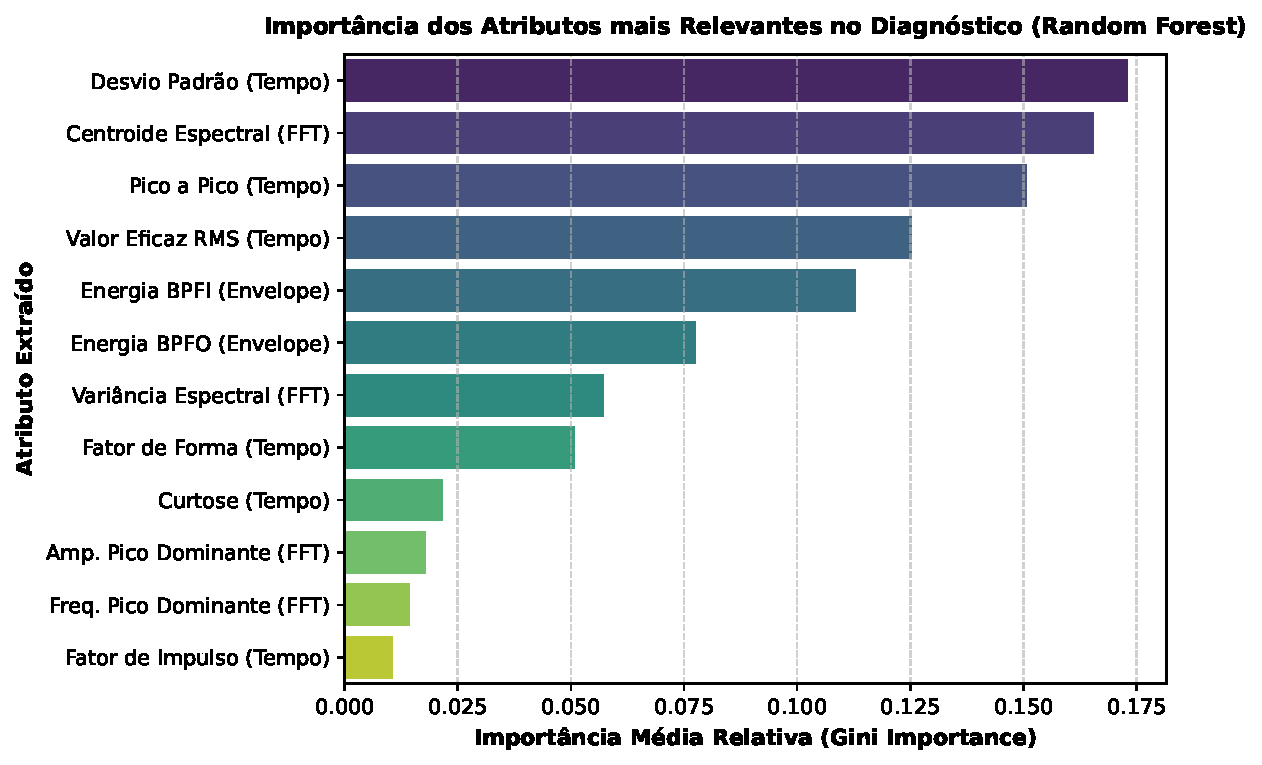
\includegraphics[width=0.88\textwidth]{fig_feature_importance.pdf}
    \caption{Classificação da importância relativa dos atributos extraídos pelo modelo Random Forest}
    \label{fig:feature_importance}
    \legend{Fonte: Elaborado pelo autor (2026).}
\end{figure}

A análise do ranking de relevância revela insights físicos fundamentais:
\begin{enumerate}
    \item \textbf{Predomínio de Métricas de Dispersão e Energia Temporal:} O Desvio Padrão ($\sigma$, \SI{17,29}{\percent}), o valor Pico a Pico ($X_{p-p}$, \SI{15,06}{\percent}) e o valor eficaz ($\text{RMS}$, \SI{12,53}{\percent}) figuram entre os quatro atributos mais discriminantes. Sob a perspectiva da dinâmica mecânica, o surgimento de descontinuidades na pista ou esferas altera drasticamente a variabilidade e a amplitude pico a pico da aceleração transmitida à carcaça do mancal, tornando essas grandezas métricas basais altamente robustas para segregar condições sadias de estados com falha;
    \item \textbf{Papel Discriminante do Centroide Espectral (\SI{16,55}{\percent}):} O centroide espectral emergiu como o segundo atributo mais relevante de todo o modelo. Conforme fundamentado na \autoref{sec:processamento_sinais}, o atrito em componentes íntegros concentra energia predominantemente em baixas frequências (desbalanceamento e desalinhamento), ao passo que impactos pontuais causados por defeitos excitam modos de alta frequência, deslocando o centro de massa espectral para patamares superiores;
    \item \textbf{Discriminação Específica de Falhas via Energia BPFI (\SI{11,29}{\percent}):} Entre os atributos espectrais fundamentados na cinemática do rolamento, a energia na banda da frequência $\text{BPFI}$ (extraída do espectro de envelope via Hilbert) apresentou a maior importância. Essa relevância decorre do fato de que falhas na pista interna são as mais desafiadoras de diagnosticar devido à modulação em amplitude com a rotação do eixo ($f_r$). O monitoramento específico da energia nessa frequência cinemática fornece a assinatura necessária para desambiguar a pista interna dos demais modos de falha.
\end{enumerate}

\section{Desempenho dos Classificadores: Random Forest vs. SVM}
\label{sec:desempenho_modelos}

\subsection{Validação Cruzada Estratificada Agrupada (Stratified Group 4-Fold)}
Para avaliar o impacto da seleção de atributos e verificar a estabilidade dos modelos na ausência de vazamento de dados, executou-se a validação cruzada agrupada em 4 dobras, confrontando quatro subconjuntos distintos de características. Os resultados consolidados estão sintetizados na \autoref{tab:cv_resumo}.

\begin{table}[htbp]
    \centering
    \caption{Comparativo de validação cruzada agrupada (4-fold) para diferentes subconjuntos de atributos}
    \label{tab:cv_resumo}
    \begin{tabular}{llccc}
        \toprule
        \textbf{Modelo} & \textbf{Subconjunto de Atributos} & \textbf{Dimensão ($p$)} & \textbf{Acurácia Média (\%)} & \textbf{F1-Score Macro} \\
        \midrule
        \multirow{4}{*}{\textbf{Random Forest}} 
        & Tempo Base & 3 & $94,70 \pm 2,40$ & \num{0,9442} \\
        & Tempo Completo & 8 & $94,98 \pm 1,75$ & \num{0,9462} \\
        & Frequência e Envelope & 8 & $99,48 \pm 0,46$ & \num{0,9947} \\
        & \textbf{Todas as Features} & \textbf{16} & $\mathbf{99,41 \pm 0,46}$ & \textbf{\num{0,9942}} \\
        \midrule
        \multirow{4}{*}{\textbf{SVM (RBF)}} 
        & Tempo Base & 3 & $91,52 \pm 7,04$ & \num{0,9105} \\
        & Tempo Completo & 8 & $91,14 \pm 8,53$ & \num{0,9061} \\
        & Frequência e Envelope & 8 & $95,10 \pm 7,52$ & \num{0,9423} \\
        & \textbf{Todas as Features} & \textbf{16} & $\mathbf{99,43 \pm 0,50}$ & \textbf{\num{0,9943}} \\
        \bottomrule
    \end{tabular}
    \legend{Fonte: Elaborado pelo autor (2026).}
\end{table}

A evolução do desempenho ao longo dos subconjuntos de atributos evidencia conclusões metodológicas cruciais:
\begin{itemize}
    \item \textbf{Insuficiência de Atributos Temporais Isolados:} Quando alimentados exclusivamente com os 3 atributos de tempo base (RMS, Curtose e Fator de Crista), tanto o Random Forest (\SI{94,70}{\percent}) quanto o SVM (\SI{91,52}{\percent}) apresentaram desempenhos inferiores e elevada oscilação entre dobras (desvio de $\pm \SI{7,04}{\percent}$ no SVM). Isso comprova que parâmetros estocásticos temporais, embora informem sobre a presença de impactos, não possuem resolução espectral suficiente para discernir com precisão a localização física do defeito em ensaios independentes;
    \item \textbf{Efeito Sinergético do Conjunto Completo:} A combinação dos 8 atributos temporais com os 8 atributos de frequência e envelope elevou a acurácia média de ambos os modelos para patamares superiores a \SI{99,4}{\percent}, reduzindo drasticamente a variabilidade entre dobras para meros $\pm \SI{0,46}{\percent}$ na Random Forest e $\pm \SI{0,50}{\percent}$ no SVM. Essa convergência demonstra que a fusão entre características estocásticas globais e parâmetros espectrais sintonizados nas frequências cinemáticas é determinante para a generalização dos classificadores.
\end{itemize}

\subsection{Avaliação no Conjunto de Teste Independente}
Após a validação cruzada, os modelos foram avaliados no conjunto de teste independente composto por 12 ensaios físicos (\num{886} janelas discretas de \SI{0,17}{\second}) nunca apresentados aos algoritmos durante o treino. A \autoref{tab:resultados_modelos} consolida as métricas detalhadas obtidas por classe e globais.

\begin{table}[htbp]
    \centering
    \caption{Desempenho comparativo dos modelos no conjunto de teste independente (886 janelas, 12 ensaios)}
    \label{tab:resultados_modelos}
    \begin{tabular}{llcccc}
        \toprule
        \textbf{Modelo} & \textbf{Condição / Métrica} & \textbf{Precisão} & \textbf{Sensibilidade (\textit{Recall})} & \textbf{F1-Score} & \textbf{Acurácia Global} \\
        \midrule
        \multirow{6}{*}{\textbf{Random Forest}} 
        & Elemento Rolante (B) & \num{0.9942} & \num{0.9718} & \num{0.9829} & \multirow{6}{*}{\textbf{\SI{99.32}{\percent}}} \\
        & Pista Interna (IR)   & \num{0.9958} & \num{0.9958} & \num{0.9958} & \\
        & Saudável (Normal)    & \num{0.9875} & \num{1.0000} & \num{0.9937} & \\
        & Pista Externa (OR)   & \num{0.9958} & \num{1.0000} & \num{0.9979} & \\
        \cmidrule(lr){2-5}
        & \textbf{Média Macro} & \num{0.9933} & \num{0.9919} & \textbf{\num{0.9926}} & \\
        & \textbf{Votação por Ensaio} & --- & --- & --- & \textbf{\SI{100.00}{\percent}} (\num{12}/\num{12}) \\
        \midrule
        \multirow{6}{*}{\textbf{SVM (RBF)}} 
        & Elemento Rolante (B) & \num{1.0000} & \num{0.9548} & \num{0.9769} & \multirow{6}{*}{\textbf{\SI{99.10}{\percent}}} \\
        & Pista Interna (IR)   & \num{0.9752} & \num{1.0000} & \num{0.9874} & \\
        & Saudável (Normal)    & \num{1.0000} & \num{1.0000} & \num{1.0000} & \\
        & Pista Externa (OR)   & \num{0.9916} & \num{1.0000} & \num{0.9958} & \\
        \cmidrule(lr){2-5}
        & \textbf{Média Macro} & \num{0.9917} & \num{0.9887} & \textbf{\num{0.9900}} & \\
        & \textbf{Votação por Ensaio} & --- & --- & --- & \textbf{\SI{100.00}{\percent}} (\num{12}/\num{12}) \\
        \bottomrule
    \end{tabular}
    \legend{Fonte: Elaborado pelo autor (2026).}
\end{table}


Conforme apresentado na \autoref{tab:resultados_modelos}, o classificador \textit{Random Forest} alcançou uma acurácia global de \SI{99,32}{\percent} e \textit{F1-Score} macro de \num{0,9926}, enquanto o SVM (\textit{kernel} RBF com padronização \textit{StandardScaler}) atingiu acurácia global de \SI{99,10}{\percent} e \textit{F1-Score} macro de \num{0,9900}. Ambas as arquiteturas apresentaram sensibilidade perfeita (\SI{100,00}{\percent}) para a condição saudável (\textit{Normal}) e para falhas de pista externa (\textit{OR}), validando a elevada confiabilidade do sistema preditivo.

\section{Análise de Erros por Tipo e Severidade de Falha}
\label{sec:analise_erros}

A distribuição detalhada dos acertos e das confusões residuais entre classes pode ser examinada através das Matrizes de Confusão normalizadas apresentadas na \autoref{fig:matrizes_confusao}.

\begin{figure}[htbp]
    \centering
    \begin{subfigure}[b]{0.48\textwidth}
        \centering
        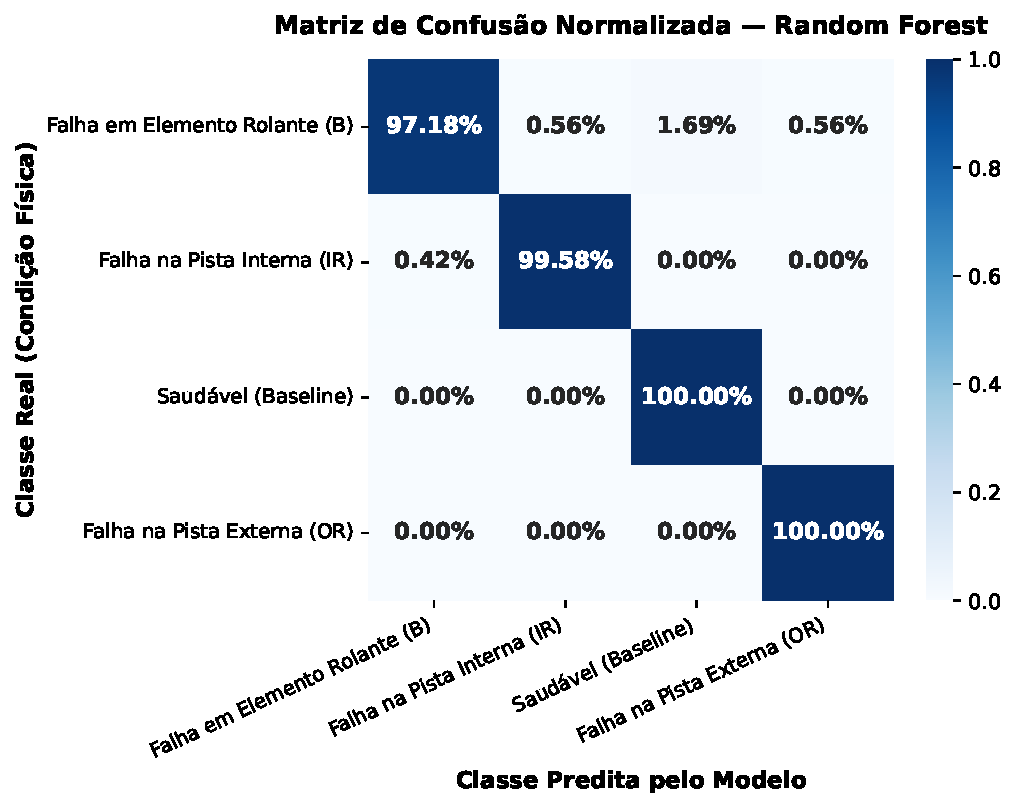
\includegraphics[width=\textwidth]{fig_matriz_confusao_rf.pdf}
        \caption{Random Forest}
        \label{fig:conf_rf}
    \end{subfigure}
    \hfill
    \begin{subfigure}[b]{0.48\textwidth}
        \centering
        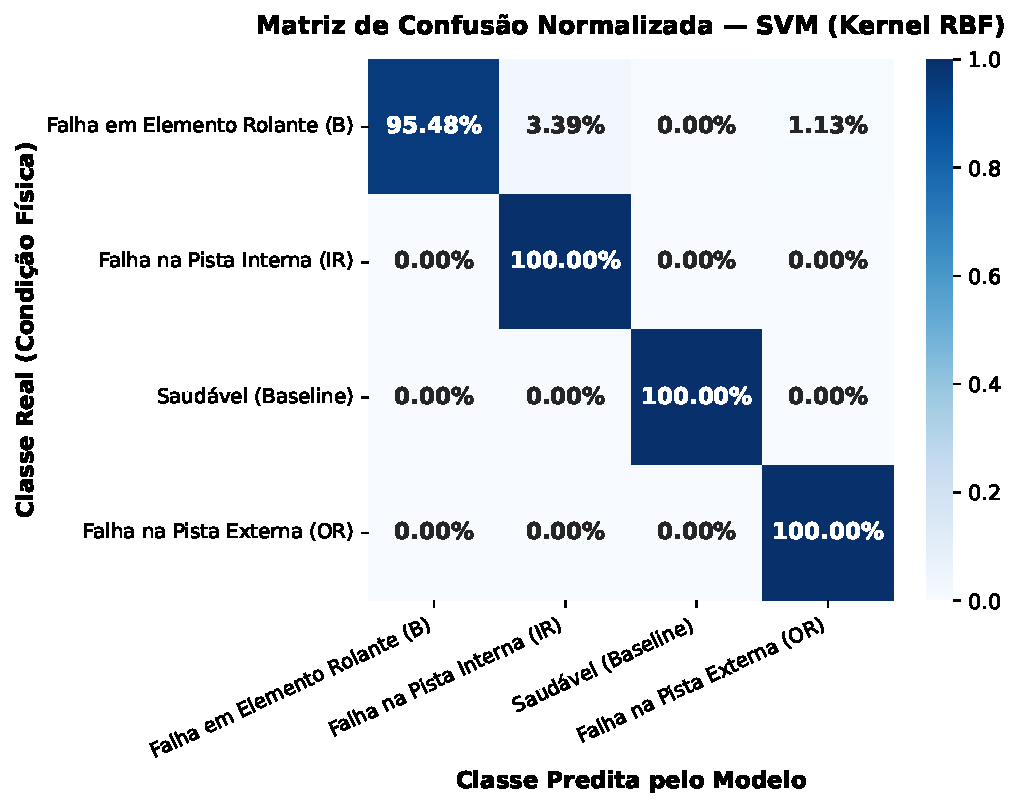
\includegraphics[width=\textwidth]{fig_matriz_confusao_svm.pdf}
        \caption{SVM (Kernel RBF)}
        \label{fig:conf_svm}
    \end{subfigure}
    \caption{Matrizes de confusão normalizadas para os modelos no conjunto de teste independente}
    \label{fig:matrizes_confusao}
    \legend{Fonte: Elaborado pelo autor (2026).}
\end{figure}

\subsection{Interpretação Mecânica do Comportamento da Classe B (Elemento Rolante)}
A observação das matrizes de confusão revela que a quase totalidade dos desvios residuais concentrou-se na classe B (defeito em elemento rolante / esfera), cujo recall situou-se em \SI{97,18}{\percent} na Random Forest e \SI{95,48}{\percent} no SVM. Registrou-se uma discreta confusão da classe B com as classes IR e OR.

Esse fenômeno possui fundamentação física rigorosa na dinâmica de contato de rolamentos:
\begin{enumerate}
    \item \textbf{Movimento Planetário Complexo:} Ao contrário das pistas interna e externa, que possuem trajetórias geométricas estritamente circulares e repetitivas em relação à zona de carga, as esferas realizam um movimento combinado de rotação em torno do próprio eixo (\textit{spin}, na frequência $\text{BSF}$) e translação orbital em torno do eixo do mancal (\textit{revolution}, na frequência $\text{FTF}$) \cite{harris2006rolling};
    \item \textbf{Rotação Não Confinada do Ponto de Defeito:} Uma cavidade ou trinca pontual localizada na superfície esférica não colide necessariamente contra as pistas no ápice da zona de carregamento a cada revolução. Dependendo da orientação instantânea do vetor de rotação da esfera e do deslizamento elasto-hidrodinâmico com o filme de lubrificante, o defeito pode cruzar a zona de carga fora do plano de contato direto com o anel. Nessas janelas temporais de transição, a intensidade mecânica do impacto é consideravelmente amortecida, gerando assinaturas transitórias mais suaves que se aproximam dos padrões de outras classes;
    \item \textbf{Severidade do Dano:} Em defeitos incipientes com diâmetro de \SI{0.007}{in}, a energia do choque no elemento rolante é substancialmente menor do que em diâmetros de \SI{0.021}{in}. Quando o rolamento opera sob carga leve (\SI{0}{\horsepower}), a compressão de contato hertziano é reduzida, atenuando os pulsos de vibração detectados pelo acelerômetro externo.
\end{enumerate}

\subsection{Eficácia da Estratégia de Votação Majoritária por Ensaio (File-Level Voting)}
A despeito dos discretos erros classificados em nível de janelas isoladas (\SI{0,17}{\second}), a aplicação da rotina de votação majoritária agregada por ensaio (\textit{file-level majority voting}, formulada na \autoref{eq:file_voting}) produziu um resultado notável:
\begin{equation}
    \text{Acurácia Global em Nível de Ensaio} = \mathbf{100,00\%} \quad (\num{12} \text{ acertos em } \num{12} \text{ ensaios avaliados})
    \label{eq:resultado_votacao}
\end{equation}

Em todos os 12 ensaios físicos que integraram o conjunto de teste independente (abrangendo 3 arquivos com defeito em esfera, 4 arquivos com defeito em pista interna, 4 arquivos com defeito em pista externa e 1 arquivo de condição saudável), a proporção de janelas corretamente classificadas pelo modelo supervisionado superou \SI{94}{\percent}. Em consequência, o consenso modal convergiu invariavelmente para a condição mecânica real em \SI{100}{\percent} dos equipamentos avaliados.

Esse resultado valida plenamente a viabilidade de transposição do modelo desenvolvido para caixas de mancal de rodeiros ferroviários reais: na prática operacional de engenharia, a decisão de manutenção é tomada a partir da observação de sequências contínuas de segundos ou minutos de operação do rodeiro, patamar no qual o método proposto demonstrou confiabilidade integral e ausência de falsos alarmes.
